\begin{figure}[H]
    \centering
    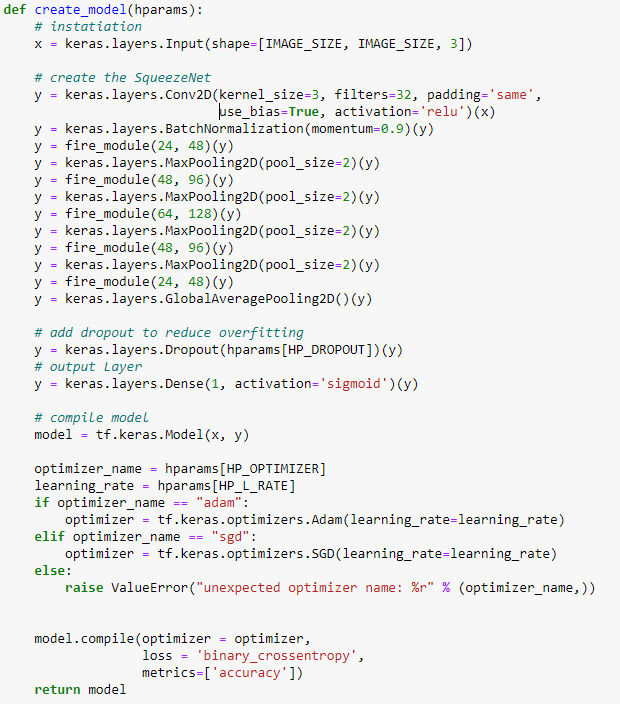
\includegraphics[width=\textwidth]{figures/squeezenet-model.png}
    \caption{The SqueezeNet model.}
    \label{fig:squeezenet-model}
\end{figure}
\begin{figure}[H]
    \centering
    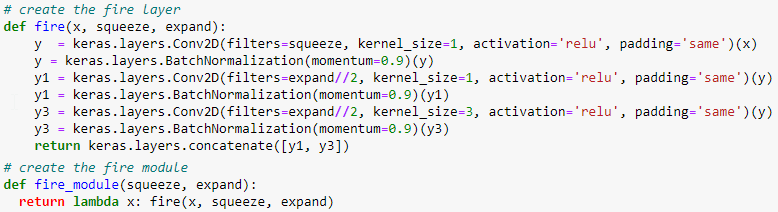
\includegraphics[width=\textwidth]{figures/squeezenet-fire-module.png}
    \caption{The fire module used in the SqueezeNet model.}
    \label{fig:squeezenet-fire-module}
\end{figure}


\begin{landscape}
\begin{table}
    \caption{SqueezeNet results after initial training on the small COVIDx-CXR dataset.}
    \centering
    \begin{tabular}{l|l|l|l|l|l|l|l|l}
    Model &  Dropout & Optimiser & Learning Rate & \begin{tabular}[c]{@{}l@{}}Mean Test\\ Accuracy\end{tabular} & \begin{tabular}[c]{@{}l@{}}Mean Test\\Precision\end{tabular} & \begin{tabular}[c]{@{}l@{}}Mean Test\\Recall\end{tabular} & \begin{tabular}[c]{@{}l@{}}Mean Test\\F1 Score\end{tabular} & \begin{tabular}[c]{@{}l@{}}Training\\ Time (s)\end{tabular} \\
    \hline\hline
    SqueezeNet & 0.2 & Adam & 0.0005 & 0.9290 & 0.9036 & 0.9620 & 0.9316 & 282 \\
    SqueezeNet & 0.1 & Adam & 0.0005 & 0.9165 & 0.8744 & 0.9750 & 0.9213 & 327 \\
    SqueezeNet & 0.2 & Adam & 0.0010 & 0.8980 & 0.9015 & 0.8980 & 0.8911 & 261 \\
    SqueezeNet & 0.1 & Adam & 0.0010 & 0.8965 & 0.8617 & 0.9530 & 0.9027 & 399 \\
    SqueezeNet & 0.1 & SGD & 0.0010 & 0.8275 & 0.7992 & 0.8860 & 0.8351 & 620 \\
    SqueezeNet & 0.1 & SGD & 0.0005 & 0.7815 & 0.7257 & 0.9060 & 0.8045 & 542 \\
    SqueezeNet & 0.2 & SGD & 0.0010 & 0.7710 & 0.7625 & 0.8370 & 0.7857 & 406 \\
    SqueezeNet & 0.2 & SGD & 0.0005 & 0.7650 & 0.7382 & 0.8430 & 0.7825 & 513
    \end{tabular}
    \label{fig:squeezenet-results}
\end{table}
\end{landscape}